%%%%%%%%%%%%%%%%%%%%%%%%%%%%%%%%%%%%%%%%%
% Short Sectioned Assignment
% LaTeX Template
% Version 1.0 (5/5/12)
%
% This template has been downloaded from:
% http://www.LaTeXTemplates.com
%
% Original author:
% Frits Wenneker (http://www.howtotex.com)
%
% License:
% CC BY-NC-SA 3.0 (http://creativecommons.org/licenses/by-nc-sa/3.0/)
%
%%%%%%%%%%%%%%%%%%%%%%%%%%%%%%%%%%%%%%%%%

%----------------------------------------------------------------------------------------
%	PACKAGES AND OTHER DOCUMENT CONFIGURATIONS
%----------------------------------------------------------------------------------------

\documentclass[paper=a4, fontsize=11pt]{scrartcl} % A4 paper and 11pt font size

\usepackage[T1]{fontenc} % Use 8-bit encoding that has 256 glyphs
\usepackage{fourier} % Use the Adobe Utopia font for the document - comment this line to return to the LaTeX default
\usepackage[english]{babel} % English language/hyphenation
\usepackage{amsmath,amsfonts,amsthm} % Math packages
\usepackage{color}
\usepackage{sectsty} % Allows customizing section commands
\usepackage{graphicx}
\allsectionsfont{\centering \normalfont\scshape} % Make all sections centered, the default font and small caps

\usepackage{fancyhdr} % Custom headers and footers
\pagestyle{fancyplain} % Makes all pages in the document conform to the custom headers and footers
\fancyhead{} % No page header - if you want one, create it in the same way as the footers below
\fancyfoot[L]{} % Empty left footer
\fancyfoot[C]{} % Empty center footer
\fancyfoot[R]{\thepage} % Page numbering for right footer
\renewcommand{\headrulewidth}{0pt} % Remove header underlines
\renewcommand{\footrulewidth}{0pt} % Remove footer underlines
\setlength{\headheight}{13.6pt} % Customize the height of the header

\numberwithin{equation}{section} % Number equations within sections (i.e. 1.1, 1.2, 2.1, 2.2 instead of 1, 2, 3, 4)
\numberwithin{figure}{section} % Number figures within sections (i.e. 1.1, 1.2, 2.1, 2.2 instead of 1, 2, 3, 4)
\numberwithin{table}{section} % Number tables within sections (i.e. 1.1, 1.2, 2.1, 2.2 instead of 1, 2, 3, 4)

\setlength\parindent{0pt} % Removes all indentation from paragraphs - comment this line for an assignment with lots of text

%----------------------------------------------------------------------------------------
%	TITLE SECTION
%----------------------------------------------------------------------------------------

\newcommand{\horrule}[1]{\rule{\linewidth}{#1}} % Create horizontal rule command with 1 argument of height

\title{	
\normalfont \normalsize 
\textsc{Max-Planck-Institute, Stuttgart} \\ [25pt] % Your university, school and/or department name(s)
\horrule{0.5pt} \\[0.4cm] % Thin top horizontal rule
\huge Chasing $d$-wave superconductivity \\
in the $2D$ Hubbard Model % The assignment title
\horrule{2pt} \\[0.5cm] % Thick bottom horizontal rule
}

\author{Ciro Taranto, Demetrio Vilardi} % Your name

\date{\normalsize\today} % Today's date or a custom date

\begin{document}

\maketitle % Print the title

%----------------------------------------------------------------------------------------
%	PROBLEM 1
%----------------------------------------------------------------------------------------

\section{Introduction}
In this report we show our DMF$^2$RG results for the  2$d$ one band Hubbard model in the intermediate-to-strong coupling regime and with a Fermi surface structure similar to the cuprate one. 
The report is structured as follows. 
First we explain the cutoff choice that we have implemented. 
Then we show our results, namely: 
\begin{itemize}
\item With full frequency dependence vertex we manage to recover the DMFT N\' eel temperature, at weak and strong coupling; 
\item The leading instability is incommensurate antiferromagetic; 
\item At strong coupling the incommensurability vector does not necessarily correspond to the one of the particle-hole bubble; 
\item Nonlocal fluctuations only slightly decrease the DMFT-N\' eel temperature; 
\item We do not find a $d$-wave pairing instability at the temperature studied; 
\item The $d$-wave pairing fluctuations can become large close to the antiferromagnetic instability, showing that the spin-fermion mechanism is active also at strong coupling. 
\end{itemize} 
In the second part of this report, we discuss several ideas and proposals that aim to a better understanding of the data obtained thus far. 
%------------------------------------------------

\section{Method and cutoff choice}
We used a \textit{local conserving cutoff}, which means that the $\Lambda$ dependence of the Green's function is chosen in such a way that the DMFT self-consistency condition is verified for every $\Lambda$-value:
\begin{equation}
\label{eq:selcon}
\int_{\mathbf{k}} G^\Lambda_{\mathbf{k},\nu}|_{\Sigma^{\mathrm{DMFT}}} = \mathcal{G}_{\nu}.   
\end{equation}
Here $\mathcal{G}_{\nu}$ is the Green's function of the Anderson Impurity model associated with the DMFT problem of the lattice system considered. The notation $|_{\Sigma^{\mathrm{DMFT}}}$ means that the Green's function is computed with the DMFT self-energy $\Sigma_\nu^{\mathrm{DMFT}}$, see below. 
The $\Lambda$-dependent Green's function is defined by: 
\begin{equation}
G_{\mathbf{k},\nu}^\Lambda = \left[i\nu+(1-\Lambda)\epsilon_{\mathbf{k}}
+\mu -
f^\Lambda_{\nu}+ \Delta_{\nu} -\Sigma_{\mathbf{k},\nu}^\Lambda
 \right]^{-1},
\end{equation}
where $\Delta_\nu$ is the hybridization function associated to the Anderson Impurity model, $\mathcal{G}_\nu=\left[i\nu-\Delta_\nu+\mu \right]^{-1}$. The function $f^\Lambda_\nu$ is fixed to guarantee equation \ref{eq:selcon}. Considering that $G$ and $\mathcal{G}$ fulfill the DMFT self-consistency condition one has $f^{\Lambda=1}_\nu=1$, $f^{\Lambda=0}_\nu=0$.  
%------------------------------------------------

\section{Results}
\subsection{Half filling at strong coupling} 
\begin{itemize}
\item Flow at strong coupling: flow of the magnetic channel+flow of the susceptibility; 
\item The N\' eel temperature can be extrapolated from the inverse of the susceptibility. 
While the N\' eel temperature is strongly reduced by the local fluctuations including nonlocal fluctuations and self-energy feedback does not reduce the temperature much further, at least in the half-filling, particle-hole symmetric case of Fig. \ref{fig:extrasusc}. Away from half-filling where also other channels come into play, the nonlocal channel competition is slightly more effective, but we never find a complete suppression of incommensurate antiferromagnetism to ascribe to nonlocal fluctuations in other channels. 

\item Magnetic channel frequency plot, at strong and weak coupling; 
\end{itemize} 
%----------------------------------------------------------------------------------------
\subsection{Away from half filling}

\begin{figure}[t!]
\begin{center}
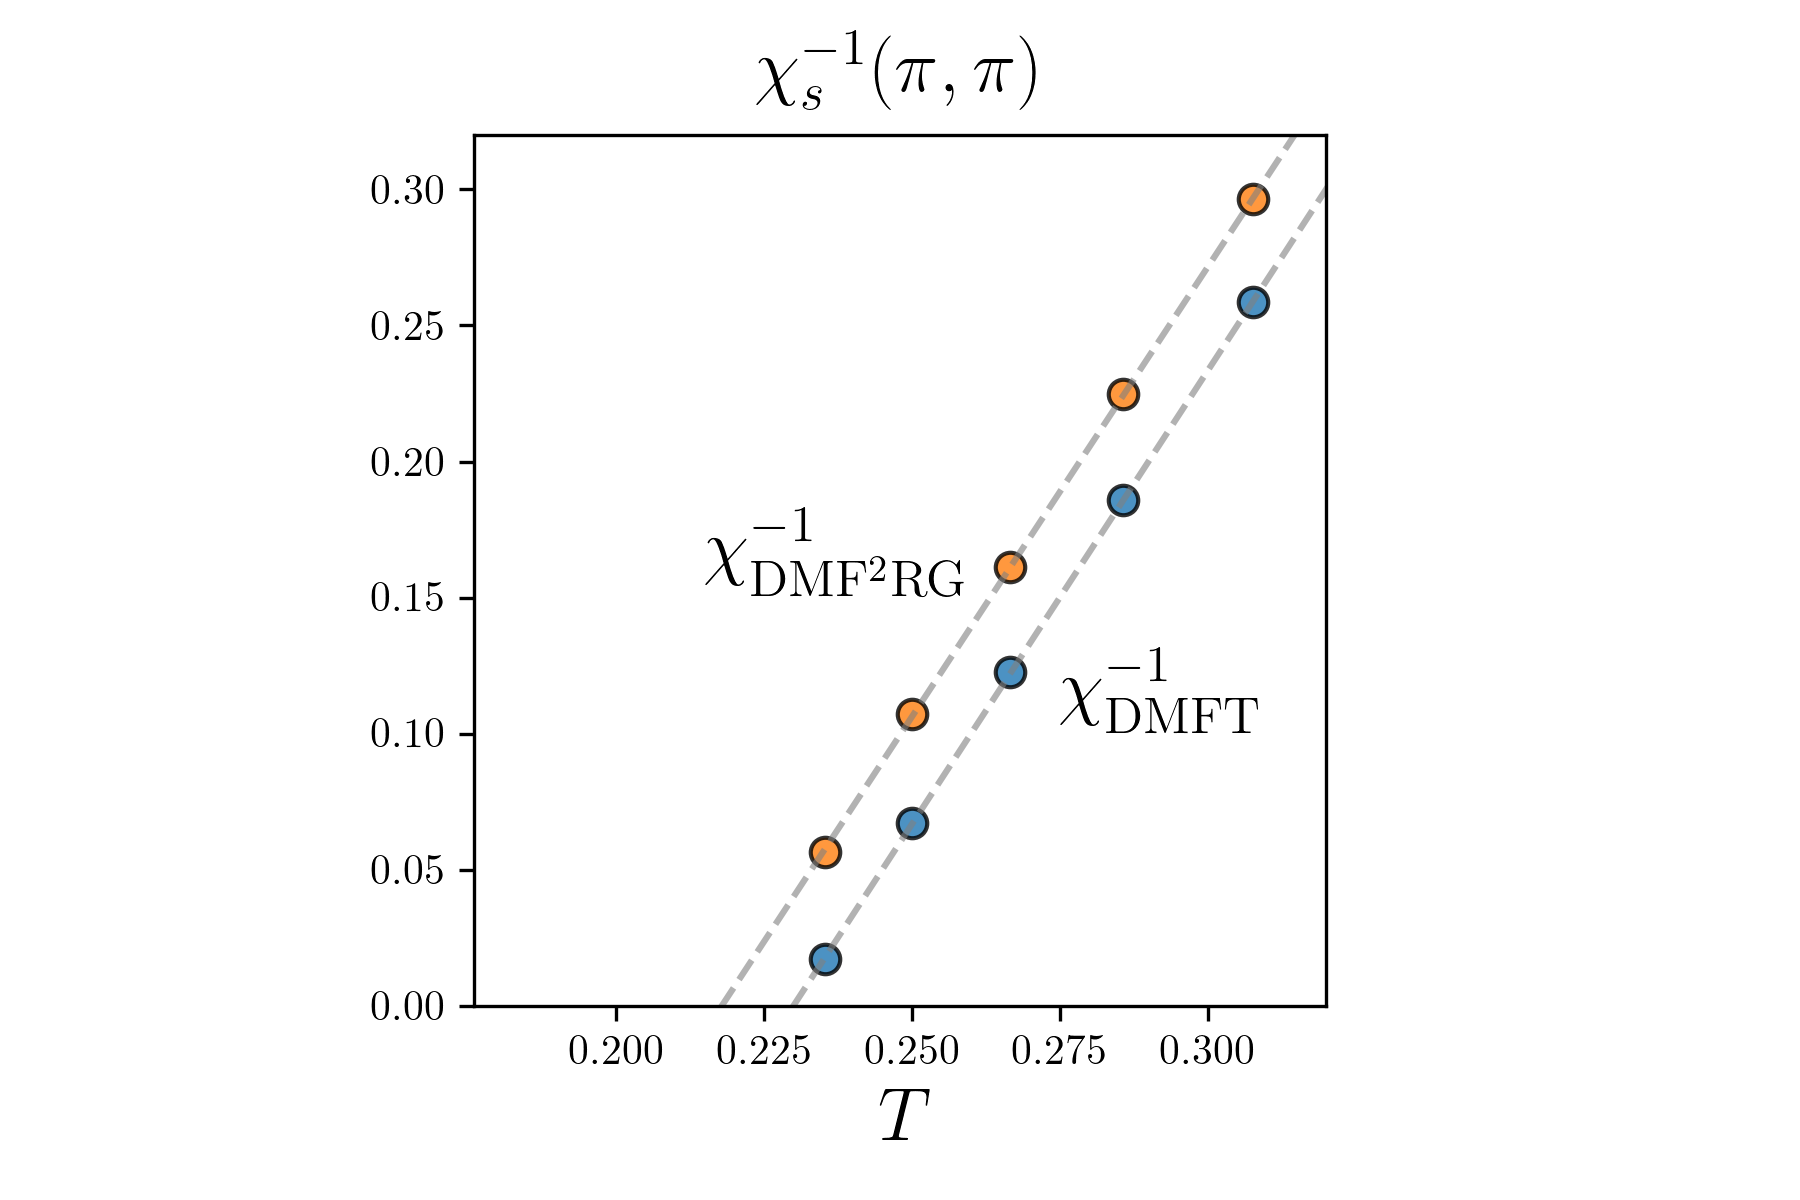
\includegraphics[width=0.8\textwidth]{plots/extrapolate_susc.png}
\caption{Critical scale and $d$-wave fluctuations for $U=8t$, $T=0.08t$ and $t'=0.2$. The orange and purple lines refer to the \textit{decoupled} case, described in the text.} 
\label{fig:phasediag} 
\end{center}
\end{figure}


\begin{itemize}
\item In Fig. \ref{fig:phasediag} we show the \textit{critical scale} for a parameter set at strong coupling ($U=8t$) and for $T=0.08t$. 
We observe that for doping values up to $\delta = 0.18$ the flow stops at a value of $\Lambda > 0$. With our cutoff choice this means that the system shows an instability when the "nonlocality" of the Green's function is further increased. 
The instability is always of the incommensurate antiferromagnetic type, with incommensurability vector that do not necessarly correspond to the maximum of the particle-hole bubble (with DMFT self-energy). 
In the same figure, we compare the critical scale with the one obtained including in the flow equations only the magnetic and the $d$-wave superconducting channel. 
We can see that suppressing the channel competition slightly increases the tendency to iAF.

More important is the study of the maximum of the $d$-wave pairing channel.
Although the numerical values are always very small ($<30t$) when compared to the leading magnetic channel, $\mathcal{O}(10^3)$, it is clear that when the magnetic fluctuations become large these drive also the values of the pairing channel. 
The strong decrease of the $d$-wave pairing for small doping, is due to the fact that we do not enter the broken symmetry phase, but stop the flow when the critical scale is reached.
To identify the mechanism responsible for the formation of the $d$-wave pairing fluctuations we compute the flow including only the magnetic and $d$-wave pairing channel. 
we can see that, by doing so, the $d$-wave pairing is further enhanced. 
To conclude: a $d$-wave instability is not observed at the temperature studied. However, $d$-wave pairing fluctuations are driven by the magnetic channel. These could lead to an instability either at lowever temperature or if one would be able to continue the flow also beyond the critical scale, or in the broken symmetry region (assuming that for some reason, or due to order parameter fluctuations beyond our method, the magnetic order is not realized).
\begin{figure}[t!]
\begin{center}
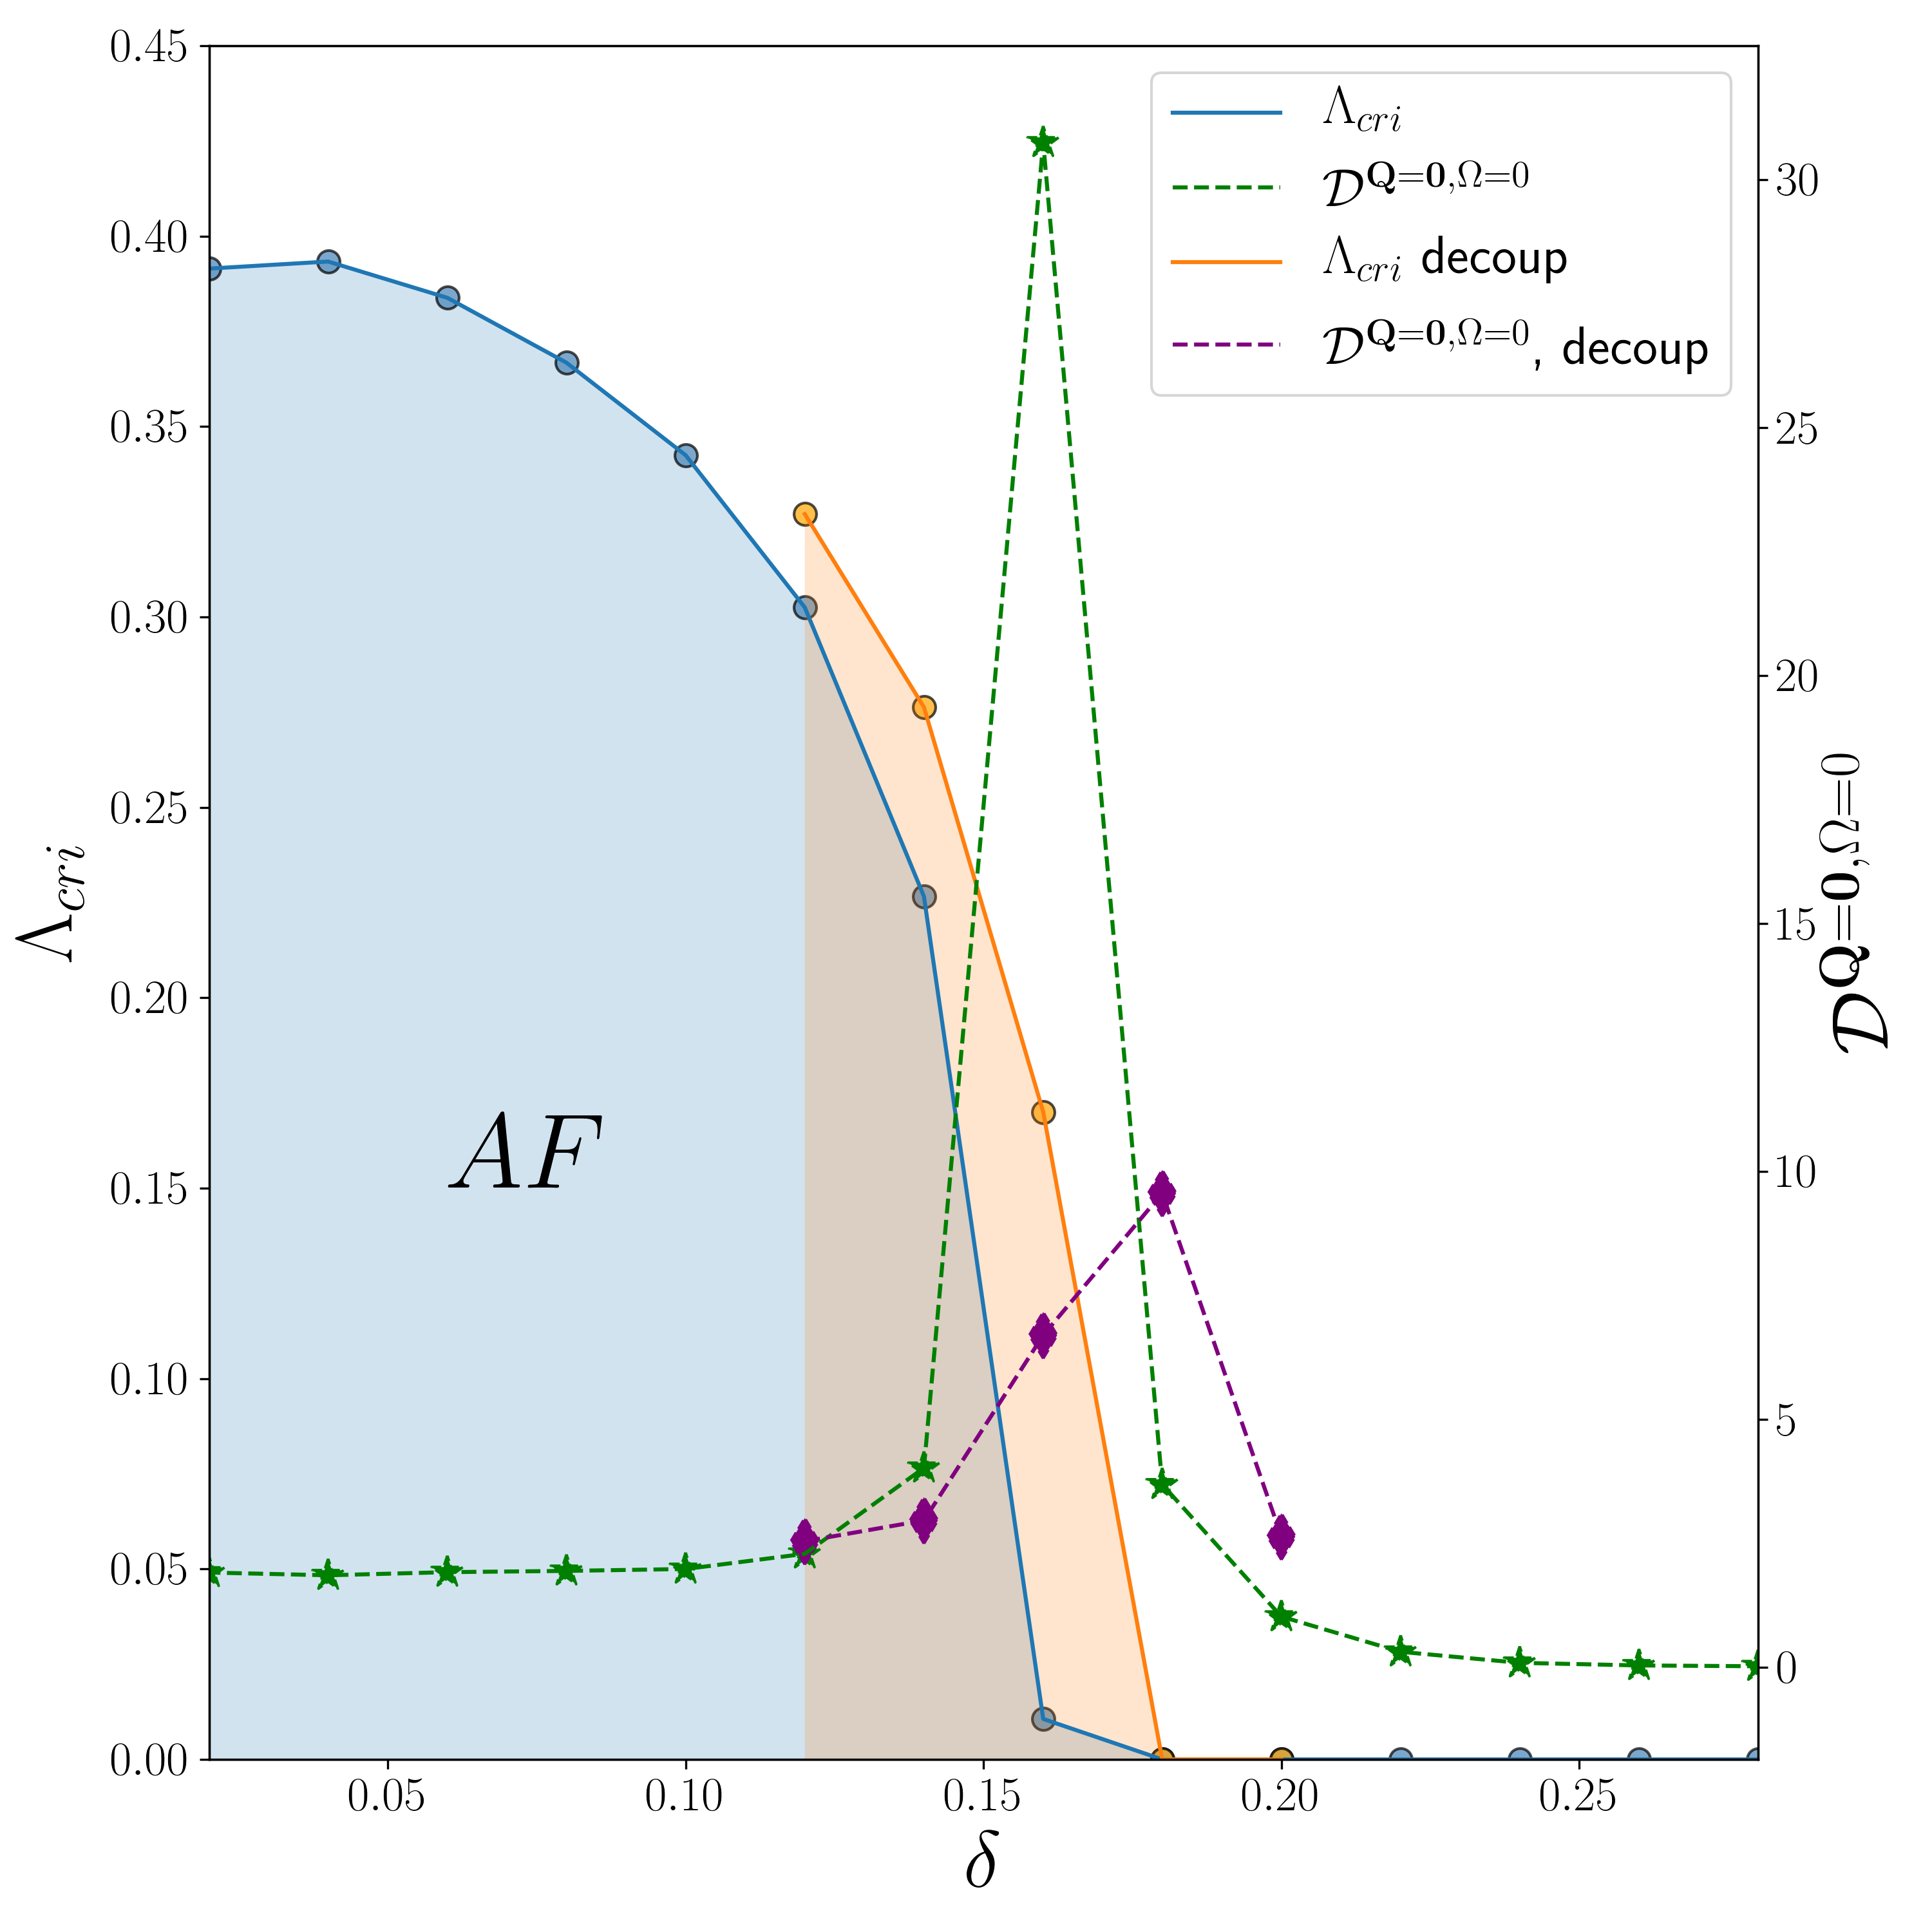
\includegraphics[width=0.8\textwidth]{plots/pairing_plus_criscale.png}
\caption{Extrapolation of the susceptibility for $U=4t$ and in the particle-hole symmetric case.} 
\label{fig:extrasusc} 
\end{center}
\end{figure}


\item flow of the d-wave channel (at different temperatures?); 
\item Perpendicular ladder, comparison of the $d$-wave in different schemes: PL, decoupled, dmf2rg; 
\end{itemize}  

%----------------------------------------------------------------------------------------
\section{Proposed investigations} 
\begin{itemize}
\item origin of $d$-wave superconductivity;  
\end{itemize} 
\newpage
\section{Rawdata and plots to get} 
{\color{red} 
\begin{itemize}
\item flow of susceptibility+flow of the magetic (strong coupling HF); \textbf{Demetrio}
\item Extrapolation of N\' eel temperature from susceptibility (with self-energy);\textbf{Ciro}  
\item Magnetic channel frequency plot, at strong and weak coupling; \textbf{Ciro+Demetrio script} 
\item doping scan at fixed temperature $\beta=50$: Critical scale and pairing fluctuations; \textbf{Ciro} 
\item flow of the d-wave channel (at different temperatures?); \textbf{Demetrio}
\item Perpendicular ladder$\rightarrow$ comparison of the $d$-wave in different schemes: PL, decoupled, dmf2rg (function of $\Lambda$ also for the Magnetic) \textbf{Demetrio};
\item Maximum of $d$-wave as function of the maximum of $\mathcal{M}$;   
\item Decoupled vs non decoupled (AF+$d$-wave fluct) Phase diagram   \textbf{Ciro} - plot of the maximum of the $d$-wave as function of the maximum of the magnetic in two different ways. $a)$ fixed doping, $b$ various dopings (final $\Lambda$) ;
\end{itemize} 
 } 
 
 \section{Ideas and proposal (easy or in progress)}  
 
 \begin{itemize}
 \item Fermi Surface at strong coupling: Is the Fermi surface prone to have hot spots, also in the presence of a relatively large self-energy? How is this important for the superconductivity. 
 \end{itemize}
 \section{Further studies (hard or to be planned)}  
\begin{itemize}
\item $d$-wave fluctuations beyond the critical scale: how to get them?  
\end{itemize} 
\end{document}